
% Default to the notebook output style

    


% Inherit from the specified cell style.




    
\documentclass[11pt]{article}

    
    
    \usepackage[T1]{fontenc}
    % Nicer default font (+ math font) than Computer Modern for most use cases
    \usepackage{mathpazo}

    % Basic figure setup, for now with no caption control since it's done
    % automatically by Pandoc (which extracts ![](path) syntax from Markdown).
    \usepackage{graphicx}
    % We will generate all images so they have a width \maxwidth. This means
    % that they will get their normal width if they fit onto the page, but
    % are scaled down if they would overflow the margins.
    \makeatletter
    \def\maxwidth{\ifdim\Gin@nat@width>\linewidth\linewidth
    \else\Gin@nat@width\fi}
    \makeatother
    \let\Oldincludegraphics\includegraphics
    % Set max figure width to be 80% of text width, for now hardcoded.
    \renewcommand{\includegraphics}[1]{\Oldincludegraphics[width=.8\maxwidth]{#1}}
    % Ensure that by default, figures have no caption (until we provide a
    % proper Figure object with a Caption API and a way to capture that
    % in the conversion process - todo).
    \usepackage{caption}
    \DeclareCaptionLabelFormat{nolabel}{}
    \captionsetup{labelformat=nolabel}

    \usepackage{adjustbox} % Used to constrain images to a maximum size 
    \usepackage{xcolor} % Allow colors to be defined
    \usepackage{enumerate} % Needed for markdown enumerations to work
    \usepackage{geometry} % Used to adjust the document margins
    \usepackage{amsmath} % Equations
    \usepackage{amssymb} % Equations
    \usepackage{textcomp} % defines textquotesingle
    % Hack from http://tex.stackexchange.com/a/47451/13684:
    \AtBeginDocument{%
        \def\PYZsq{\textquotesingle}% Upright quotes in Pygmentized code
    }
    \usepackage{upquote} % Upright quotes for verbatim code
    \usepackage{eurosym} % defines \euro
    \usepackage[mathletters]{ucs} % Extended unicode (utf-8) support
    \usepackage[utf8x]{inputenc} % Allow utf-8 characters in the tex document
    \usepackage{fancyvrb} % verbatim replacement that allows latex
    \usepackage{grffile} % extends the file name processing of package graphics 
                         % to support a larger range 
    % The hyperref package gives us a pdf with properly built
    % internal navigation ('pdf bookmarks' for the table of contents,
    % internal cross-reference links, web links for URLs, etc.)
    \usepackage{hyperref}
    \usepackage{longtable} % longtable support required by pandoc >1.10
    \usepackage{booktabs}  % table support for pandoc > 1.12.2
    \usepackage[inline]{enumitem} % IRkernel/repr support (it uses the enumerate* environment)
    \usepackage[normalem]{ulem} % ulem is needed to support strikethroughs (\sout)
                                % normalem makes italics be italics, not underlines
    

    
    
    % Colors for the hyperref package
    \definecolor{urlcolor}{rgb}{0,.145,.698}
    \definecolor{linkcolor}{rgb}{.71,0.21,0.01}
    \definecolor{citecolor}{rgb}{.12,.54,.11}

    % ANSI colors
    \definecolor{ansi-black}{HTML}{3E424D}
    \definecolor{ansi-black-intense}{HTML}{282C36}
    \definecolor{ansi-red}{HTML}{E75C58}
    \definecolor{ansi-red-intense}{HTML}{B22B31}
    \definecolor{ansi-green}{HTML}{00A250}
    \definecolor{ansi-green-intense}{HTML}{007427}
    \definecolor{ansi-yellow}{HTML}{DDB62B}
    \definecolor{ansi-yellow-intense}{HTML}{B27D12}
    \definecolor{ansi-blue}{HTML}{208FFB}
    \definecolor{ansi-blue-intense}{HTML}{0065CA}
    \definecolor{ansi-magenta}{HTML}{D160C4}
    \definecolor{ansi-magenta-intense}{HTML}{A03196}
    \definecolor{ansi-cyan}{HTML}{60C6C8}
    \definecolor{ansi-cyan-intense}{HTML}{258F8F}
    \definecolor{ansi-white}{HTML}{C5C1B4}
    \definecolor{ansi-white-intense}{HTML}{A1A6B2}

    % commands and environments needed by pandoc snippets
    % extracted from the output of `pandoc -s`
    \providecommand{\tightlist}{%
      \setlength{\itemsep}{0pt}\setlength{\parskip}{0pt}}
    \DefineVerbatimEnvironment{Highlighting}{Verbatim}{commandchars=\\\{\}}
    % Add ',fontsize=\small' for more characters per line
    \newenvironment{Shaded}{}{}
    \newcommand{\KeywordTok}[1]{\textcolor[rgb]{0.00,0.44,0.13}{\textbf{{#1}}}}
    \newcommand{\DataTypeTok}[1]{\textcolor[rgb]{0.56,0.13,0.00}{{#1}}}
    \newcommand{\DecValTok}[1]{\textcolor[rgb]{0.25,0.63,0.44}{{#1}}}
    \newcommand{\BaseNTok}[1]{\textcolor[rgb]{0.25,0.63,0.44}{{#1}}}
    \newcommand{\FloatTok}[1]{\textcolor[rgb]{0.25,0.63,0.44}{{#1}}}
    \newcommand{\CharTok}[1]{\textcolor[rgb]{0.25,0.44,0.63}{{#1}}}
    \newcommand{\StringTok}[1]{\textcolor[rgb]{0.25,0.44,0.63}{{#1}}}
    \newcommand{\CommentTok}[1]{\textcolor[rgb]{0.38,0.63,0.69}{\textit{{#1}}}}
    \newcommand{\OtherTok}[1]{\textcolor[rgb]{0.00,0.44,0.13}{{#1}}}
    \newcommand{\AlertTok}[1]{\textcolor[rgb]{1.00,0.00,0.00}{\textbf{{#1}}}}
    \newcommand{\FunctionTok}[1]{\textcolor[rgb]{0.02,0.16,0.49}{{#1}}}
    \newcommand{\RegionMarkerTok}[1]{{#1}}
    \newcommand{\ErrorTok}[1]{\textcolor[rgb]{1.00,0.00,0.00}{\textbf{{#1}}}}
    \newcommand{\NormalTok}[1]{{#1}}
    
    % Additional commands for more recent versions of Pandoc
    \newcommand{\ConstantTok}[1]{\textcolor[rgb]{0.53,0.00,0.00}{{#1}}}
    \newcommand{\SpecialCharTok}[1]{\textcolor[rgb]{0.25,0.44,0.63}{{#1}}}
    \newcommand{\VerbatimStringTok}[1]{\textcolor[rgb]{0.25,0.44,0.63}{{#1}}}
    \newcommand{\SpecialStringTok}[1]{\textcolor[rgb]{0.73,0.40,0.53}{{#1}}}
    \newcommand{\ImportTok}[1]{{#1}}
    \newcommand{\DocumentationTok}[1]{\textcolor[rgb]{0.73,0.13,0.13}{\textit{{#1}}}}
    \newcommand{\AnnotationTok}[1]{\textcolor[rgb]{0.38,0.63,0.69}{\textbf{\textit{{#1}}}}}
    \newcommand{\CommentVarTok}[1]{\textcolor[rgb]{0.38,0.63,0.69}{\textbf{\textit{{#1}}}}}
    \newcommand{\VariableTok}[1]{\textcolor[rgb]{0.10,0.09,0.49}{{#1}}}
    \newcommand{\ControlFlowTok}[1]{\textcolor[rgb]{0.00,0.44,0.13}{\textbf{{#1}}}}
    \newcommand{\OperatorTok}[1]{\textcolor[rgb]{0.40,0.40,0.40}{{#1}}}
    \newcommand{\BuiltInTok}[1]{{#1}}
    \newcommand{\ExtensionTok}[1]{{#1}}
    \newcommand{\PreprocessorTok}[1]{\textcolor[rgb]{0.74,0.48,0.00}{{#1}}}
    \newcommand{\AttributeTok}[1]{\textcolor[rgb]{0.49,0.56,0.16}{{#1}}}
    \newcommand{\InformationTok}[1]{\textcolor[rgb]{0.38,0.63,0.69}{\textbf{\textit{{#1}}}}}
    \newcommand{\WarningTok}[1]{\textcolor[rgb]{0.38,0.63,0.69}{\textbf{\textit{{#1}}}}}
    
    
    % Define a nice break command that doesn't care if a line doesn't already
    % exist.
    \def\br{\hspace*{\fill} \\* }
    % Math Jax compatability definitions
    \def\gt{>}
    \def\lt{<}
    % Document parameters
    \title{Python R training course - Session 4}
    
    
    

    % Pygments definitions
    
\makeatletter
\def\PY@reset{\let\PY@it=\relax \let\PY@bf=\relax%
    \let\PY@ul=\relax \let\PY@tc=\relax%
    \let\PY@bc=\relax \let\PY@ff=\relax}
\def\PY@tok#1{\csname PY@tok@#1\endcsname}
\def\PY@toks#1+{\ifx\relax#1\empty\else%
    \PY@tok{#1}\expandafter\PY@toks\fi}
\def\PY@do#1{\PY@bc{\PY@tc{\PY@ul{%
    \PY@it{\PY@bf{\PY@ff{#1}}}}}}}
\def\PY#1#2{\PY@reset\PY@toks#1+\relax+\PY@do{#2}}

\expandafter\def\csname PY@tok@gd\endcsname{\def\PY@tc##1{\textcolor[rgb]{0.63,0.00,0.00}{##1}}}
\expandafter\def\csname PY@tok@gu\endcsname{\let\PY@bf=\textbf\def\PY@tc##1{\textcolor[rgb]{0.50,0.00,0.50}{##1}}}
\expandafter\def\csname PY@tok@gt\endcsname{\def\PY@tc##1{\textcolor[rgb]{0.00,0.27,0.87}{##1}}}
\expandafter\def\csname PY@tok@gs\endcsname{\let\PY@bf=\textbf}
\expandafter\def\csname PY@tok@gr\endcsname{\def\PY@tc##1{\textcolor[rgb]{1.00,0.00,0.00}{##1}}}
\expandafter\def\csname PY@tok@cm\endcsname{\let\PY@it=\textit\def\PY@tc##1{\textcolor[rgb]{0.25,0.50,0.50}{##1}}}
\expandafter\def\csname PY@tok@vg\endcsname{\def\PY@tc##1{\textcolor[rgb]{0.10,0.09,0.49}{##1}}}
\expandafter\def\csname PY@tok@vi\endcsname{\def\PY@tc##1{\textcolor[rgb]{0.10,0.09,0.49}{##1}}}
\expandafter\def\csname PY@tok@vm\endcsname{\def\PY@tc##1{\textcolor[rgb]{0.10,0.09,0.49}{##1}}}
\expandafter\def\csname PY@tok@mh\endcsname{\def\PY@tc##1{\textcolor[rgb]{0.40,0.40,0.40}{##1}}}
\expandafter\def\csname PY@tok@cs\endcsname{\let\PY@it=\textit\def\PY@tc##1{\textcolor[rgb]{0.25,0.50,0.50}{##1}}}
\expandafter\def\csname PY@tok@ge\endcsname{\let\PY@it=\textit}
\expandafter\def\csname PY@tok@vc\endcsname{\def\PY@tc##1{\textcolor[rgb]{0.10,0.09,0.49}{##1}}}
\expandafter\def\csname PY@tok@il\endcsname{\def\PY@tc##1{\textcolor[rgb]{0.40,0.40,0.40}{##1}}}
\expandafter\def\csname PY@tok@go\endcsname{\def\PY@tc##1{\textcolor[rgb]{0.53,0.53,0.53}{##1}}}
\expandafter\def\csname PY@tok@cp\endcsname{\def\PY@tc##1{\textcolor[rgb]{0.74,0.48,0.00}{##1}}}
\expandafter\def\csname PY@tok@gi\endcsname{\def\PY@tc##1{\textcolor[rgb]{0.00,0.63,0.00}{##1}}}
\expandafter\def\csname PY@tok@gh\endcsname{\let\PY@bf=\textbf\def\PY@tc##1{\textcolor[rgb]{0.00,0.00,0.50}{##1}}}
\expandafter\def\csname PY@tok@ni\endcsname{\let\PY@bf=\textbf\def\PY@tc##1{\textcolor[rgb]{0.60,0.60,0.60}{##1}}}
\expandafter\def\csname PY@tok@nl\endcsname{\def\PY@tc##1{\textcolor[rgb]{0.63,0.63,0.00}{##1}}}
\expandafter\def\csname PY@tok@nn\endcsname{\let\PY@bf=\textbf\def\PY@tc##1{\textcolor[rgb]{0.00,0.00,1.00}{##1}}}
\expandafter\def\csname PY@tok@no\endcsname{\def\PY@tc##1{\textcolor[rgb]{0.53,0.00,0.00}{##1}}}
\expandafter\def\csname PY@tok@na\endcsname{\def\PY@tc##1{\textcolor[rgb]{0.49,0.56,0.16}{##1}}}
\expandafter\def\csname PY@tok@nb\endcsname{\def\PY@tc##1{\textcolor[rgb]{0.00,0.50,0.00}{##1}}}
\expandafter\def\csname PY@tok@nc\endcsname{\let\PY@bf=\textbf\def\PY@tc##1{\textcolor[rgb]{0.00,0.00,1.00}{##1}}}
\expandafter\def\csname PY@tok@nd\endcsname{\def\PY@tc##1{\textcolor[rgb]{0.67,0.13,1.00}{##1}}}
\expandafter\def\csname PY@tok@ne\endcsname{\let\PY@bf=\textbf\def\PY@tc##1{\textcolor[rgb]{0.82,0.25,0.23}{##1}}}
\expandafter\def\csname PY@tok@nf\endcsname{\def\PY@tc##1{\textcolor[rgb]{0.00,0.00,1.00}{##1}}}
\expandafter\def\csname PY@tok@si\endcsname{\let\PY@bf=\textbf\def\PY@tc##1{\textcolor[rgb]{0.73,0.40,0.53}{##1}}}
\expandafter\def\csname PY@tok@s2\endcsname{\def\PY@tc##1{\textcolor[rgb]{0.73,0.13,0.13}{##1}}}
\expandafter\def\csname PY@tok@nt\endcsname{\let\PY@bf=\textbf\def\PY@tc##1{\textcolor[rgb]{0.00,0.50,0.00}{##1}}}
\expandafter\def\csname PY@tok@nv\endcsname{\def\PY@tc##1{\textcolor[rgb]{0.10,0.09,0.49}{##1}}}
\expandafter\def\csname PY@tok@s1\endcsname{\def\PY@tc##1{\textcolor[rgb]{0.73,0.13,0.13}{##1}}}
\expandafter\def\csname PY@tok@dl\endcsname{\def\PY@tc##1{\textcolor[rgb]{0.73,0.13,0.13}{##1}}}
\expandafter\def\csname PY@tok@ch\endcsname{\let\PY@it=\textit\def\PY@tc##1{\textcolor[rgb]{0.25,0.50,0.50}{##1}}}
\expandafter\def\csname PY@tok@m\endcsname{\def\PY@tc##1{\textcolor[rgb]{0.40,0.40,0.40}{##1}}}
\expandafter\def\csname PY@tok@gp\endcsname{\let\PY@bf=\textbf\def\PY@tc##1{\textcolor[rgb]{0.00,0.00,0.50}{##1}}}
\expandafter\def\csname PY@tok@sh\endcsname{\def\PY@tc##1{\textcolor[rgb]{0.73,0.13,0.13}{##1}}}
\expandafter\def\csname PY@tok@ow\endcsname{\let\PY@bf=\textbf\def\PY@tc##1{\textcolor[rgb]{0.67,0.13,1.00}{##1}}}
\expandafter\def\csname PY@tok@sx\endcsname{\def\PY@tc##1{\textcolor[rgb]{0.00,0.50,0.00}{##1}}}
\expandafter\def\csname PY@tok@bp\endcsname{\def\PY@tc##1{\textcolor[rgb]{0.00,0.50,0.00}{##1}}}
\expandafter\def\csname PY@tok@c1\endcsname{\let\PY@it=\textit\def\PY@tc##1{\textcolor[rgb]{0.25,0.50,0.50}{##1}}}
\expandafter\def\csname PY@tok@fm\endcsname{\def\PY@tc##1{\textcolor[rgb]{0.00,0.00,1.00}{##1}}}
\expandafter\def\csname PY@tok@o\endcsname{\def\PY@tc##1{\textcolor[rgb]{0.40,0.40,0.40}{##1}}}
\expandafter\def\csname PY@tok@kc\endcsname{\let\PY@bf=\textbf\def\PY@tc##1{\textcolor[rgb]{0.00,0.50,0.00}{##1}}}
\expandafter\def\csname PY@tok@c\endcsname{\let\PY@it=\textit\def\PY@tc##1{\textcolor[rgb]{0.25,0.50,0.50}{##1}}}
\expandafter\def\csname PY@tok@mf\endcsname{\def\PY@tc##1{\textcolor[rgb]{0.40,0.40,0.40}{##1}}}
\expandafter\def\csname PY@tok@err\endcsname{\def\PY@bc##1{\setlength{\fboxsep}{0pt}\fcolorbox[rgb]{1.00,0.00,0.00}{1,1,1}{\strut ##1}}}
\expandafter\def\csname PY@tok@mb\endcsname{\def\PY@tc##1{\textcolor[rgb]{0.40,0.40,0.40}{##1}}}
\expandafter\def\csname PY@tok@ss\endcsname{\def\PY@tc##1{\textcolor[rgb]{0.10,0.09,0.49}{##1}}}
\expandafter\def\csname PY@tok@sr\endcsname{\def\PY@tc##1{\textcolor[rgb]{0.73,0.40,0.53}{##1}}}
\expandafter\def\csname PY@tok@mo\endcsname{\def\PY@tc##1{\textcolor[rgb]{0.40,0.40,0.40}{##1}}}
\expandafter\def\csname PY@tok@kd\endcsname{\let\PY@bf=\textbf\def\PY@tc##1{\textcolor[rgb]{0.00,0.50,0.00}{##1}}}
\expandafter\def\csname PY@tok@mi\endcsname{\def\PY@tc##1{\textcolor[rgb]{0.40,0.40,0.40}{##1}}}
\expandafter\def\csname PY@tok@kn\endcsname{\let\PY@bf=\textbf\def\PY@tc##1{\textcolor[rgb]{0.00,0.50,0.00}{##1}}}
\expandafter\def\csname PY@tok@cpf\endcsname{\let\PY@it=\textit\def\PY@tc##1{\textcolor[rgb]{0.25,0.50,0.50}{##1}}}
\expandafter\def\csname PY@tok@kr\endcsname{\let\PY@bf=\textbf\def\PY@tc##1{\textcolor[rgb]{0.00,0.50,0.00}{##1}}}
\expandafter\def\csname PY@tok@s\endcsname{\def\PY@tc##1{\textcolor[rgb]{0.73,0.13,0.13}{##1}}}
\expandafter\def\csname PY@tok@kp\endcsname{\def\PY@tc##1{\textcolor[rgb]{0.00,0.50,0.00}{##1}}}
\expandafter\def\csname PY@tok@w\endcsname{\def\PY@tc##1{\textcolor[rgb]{0.73,0.73,0.73}{##1}}}
\expandafter\def\csname PY@tok@kt\endcsname{\def\PY@tc##1{\textcolor[rgb]{0.69,0.00,0.25}{##1}}}
\expandafter\def\csname PY@tok@sc\endcsname{\def\PY@tc##1{\textcolor[rgb]{0.73,0.13,0.13}{##1}}}
\expandafter\def\csname PY@tok@sb\endcsname{\def\PY@tc##1{\textcolor[rgb]{0.73,0.13,0.13}{##1}}}
\expandafter\def\csname PY@tok@sa\endcsname{\def\PY@tc##1{\textcolor[rgb]{0.73,0.13,0.13}{##1}}}
\expandafter\def\csname PY@tok@k\endcsname{\let\PY@bf=\textbf\def\PY@tc##1{\textcolor[rgb]{0.00,0.50,0.00}{##1}}}
\expandafter\def\csname PY@tok@se\endcsname{\let\PY@bf=\textbf\def\PY@tc##1{\textcolor[rgb]{0.73,0.40,0.13}{##1}}}
\expandafter\def\csname PY@tok@sd\endcsname{\let\PY@it=\textit\def\PY@tc##1{\textcolor[rgb]{0.73,0.13,0.13}{##1}}}

\def\PYZbs{\char`\\}
\def\PYZus{\char`\_}
\def\PYZob{\char`\{}
\def\PYZcb{\char`\}}
\def\PYZca{\char`\^}
\def\PYZam{\char`\&}
\def\PYZlt{\char`\<}
\def\PYZgt{\char`\>}
\def\PYZsh{\char`\#}
\def\PYZpc{\char`\%}
\def\PYZdl{\char`\$}
\def\PYZhy{\char`\-}
\def\PYZsq{\char`\'}
\def\PYZdq{\char`\"}
\def\PYZti{\char`\~}
% for compatibility with earlier versions
\def\PYZat{@}
\def\PYZlb{[}
\def\PYZrb{]}
\makeatother


    % Exact colors from NB
    \definecolor{incolor}{rgb}{0.0, 0.0, 0.5}
    \definecolor{outcolor}{rgb}{0.545, 0.0, 0.0}



    
    % Prevent overflowing lines due to hard-to-break entities
    \sloppy 
    % Setup hyperref package
    \hypersetup{
      breaklinks=true,  % so long urls are correctly broken across lines
      colorlinks=true,
      urlcolor=urlcolor,
      linkcolor=linkcolor,
      citecolor=citecolor,
      }
    % Slightly bigger margins than the latex defaults
    
    \geometry{verbose,tmargin=1in,bmargin=1in,lmargin=1in,rmargin=1in}
    
    

    \begin{document}
    
    
    \maketitle
    
    

    
    \textbf{Lecture list}

\begin{enumerate}
\def\labelenumi{\arabic{enumi}.}
\item
  Introduction to Python
\item
  The Python Standard Library, if/loops statements
\item
  Vector/matrix structures, \texttt{numpy} library
\item
  \textbf{Python data types, File Processing, \texttt{Pandas} library}

  \begin{itemize}
  \tightlist
  \item
    Structure of Python files. Read/create a file.
  \item
    Read csv file using \texttt{Pandas} library
  \end{itemize}
\item
  Functions in Python, Debugging.
\item
  Introduction to R, R for Python programmers.
\item
  Import data, plot data.
\item
  Data Mining in Python/R.
\end{enumerate}

    \section{File Processing}\label{file-processing}

Python provides basic functions and methods necessary to manipulate
files by default. You can do most of the file manipulation using a file
object.

\subsection{Opening and Closing Files}\label{opening-and-closing-files}

Before you can read or write a file, you have to open it using Python's
built-in \textbf{open()} function. This function creates a file object,
which would be utilized to call other support methods associated with
it.

\begin{Shaded}
\begin{Highlighting}[]
\NormalTok{f }\OperatorTok{=} \BuiltInTok{open}\NormalTok{(file_name [, access_mode][, buffering])}
\end{Highlighting}
\end{Shaded}

\begin{itemize}
\tightlist
\item
  \textbf{file\_name}: The file\_name argument is a string value that
  contains the name of the file that you want to access.
\item
  \textbf{access\_mode}: The access\_mode determines the mode in which
  the file has to be opened, i.e., read, write, append, etc. A complete
  list of possible values is given below in the table. This is optional
  parameter and the default file access mode is read (r).
\item
  \textbf{buffering}: If the buffering value is set to 0, no buffering
  takes place. If the buffering value is 1, line buffering is performed
  while accessing a file. If you specify the buffering value as an
  integer greater than 1, then buffering action is performed with the
  indicated buffer size. If negative, the buffer size is the system
  default(default behavior).
\end{itemize}

Here is a list of the different modes of opening a file:

\begin{longtable}[]{@{}ll@{}}
\toprule
\begin{minipage}[b]{0.03\columnwidth}\raggedright\strut
Modes\strut
\end{minipage} & \begin{minipage}[b]{0.91\columnwidth}\raggedright\strut
Description\strut
\end{minipage}\tabularnewline
\midrule
\endhead
\begin{minipage}[t]{0.03\columnwidth}\raggedright\strut
r\strut
\end{minipage} & \begin{minipage}[t]{0.91\columnwidth}\raggedright\strut
Opens a file for reading only. The file pointer is placed at the
beginning of the file. This is the default mode.\strut
\end{minipage}\tabularnewline
\begin{minipage}[t]{0.03\columnwidth}\raggedright\strut
rb\strut
\end{minipage} & \begin{minipage}[t]{0.91\columnwidth}\raggedright\strut
Opens a file for reading only in binary format. The file pointer is
placed at the beginning of the file. This is the default mode.\strut
\end{minipage}\tabularnewline
\begin{minipage}[t]{0.03\columnwidth}\raggedright\strut
r+\strut
\end{minipage} & \begin{minipage}[t]{0.91\columnwidth}\raggedright\strut
Opens a file for both reading and writing. The file pointer placed at
the beginning of the file.\strut
\end{minipage}\tabularnewline
\begin{minipage}[t]{0.03\columnwidth}\raggedright\strut
rb+\strut
\end{minipage} & \begin{minipage}[t]{0.91\columnwidth}\raggedright\strut
Opens a file for both reading and writing in binary format. The file
pointer placed at the beginning of the file.\strut
\end{minipage}\tabularnewline
\begin{minipage}[t]{0.03\columnwidth}\raggedright\strut
w\strut
\end{minipage} & \begin{minipage}[t]{0.91\columnwidth}\raggedright\strut
Opens a file for writing only. Overwrites the file if the file exists.
If the file does not exist, creates a new file for writing.\strut
\end{minipage}\tabularnewline
\begin{minipage}[t]{0.03\columnwidth}\raggedright\strut
wb\strut
\end{minipage} & \begin{minipage}[t]{0.91\columnwidth}\raggedright\strut
Opens a file for writing only in binary format. Overwrites the file if
the file exists. If the file does not exist, creates a new file for
writing.\strut
\end{minipage}\tabularnewline
\begin{minipage}[t]{0.03\columnwidth}\raggedright\strut
w+\strut
\end{minipage} & \begin{minipage}[t]{0.91\columnwidth}\raggedright\strut
Opens a file for both writing and reading. Overwrites the existing file
if the file exists. If the file does not exist, creates a new file for
reading and writing.\strut
\end{minipage}\tabularnewline
\begin{minipage}[t]{0.03\columnwidth}\raggedright\strut
wb+\strut
\end{minipage} & \begin{minipage}[t]{0.91\columnwidth}\raggedright\strut
Opens a file for both writing and reading in binary format. Overwrites
the existing file if the file exists. If the file does not exist,
creates a new file for reading and writing.\strut
\end{minipage}\tabularnewline
\begin{minipage}[t]{0.03\columnwidth}\raggedright\strut
a\strut
\end{minipage} & \begin{minipage}[t]{0.91\columnwidth}\raggedright\strut
Opens a file for appending. The file pointer is at the end of the file
if the file exists. That is, the file is in the append mode. If the file
does not exist, it creates a new file for writing.\strut
\end{minipage}\tabularnewline
\begin{minipage}[t]{0.03\columnwidth}\raggedright\strut
ab\strut
\end{minipage} & \begin{minipage}[t]{0.91\columnwidth}\raggedright\strut
Opens a file for appending in binary format. The file pointer is at the
end of the file if the file exists. That is, the file is in the append
mode. If the file does not exist, it creates a new file for
writing.\strut
\end{minipage}\tabularnewline
\begin{minipage}[t]{0.03\columnwidth}\raggedright\strut
a+\strut
\end{minipage} & \begin{minipage}[t]{0.91\columnwidth}\raggedright\strut
Opens a file for both appending and reading. The file pointer is at the
end of the file if the file exists. The file opens in the append mode.
If the file does not exist, it creates a new file for reading and
writing.\strut
\end{minipage}\tabularnewline
\begin{minipage}[t]{0.03\columnwidth}\raggedright\strut
ab+\strut
\end{minipage} & \begin{minipage}[t]{0.91\columnwidth}\raggedright\strut
Opens a file for both appending and reading in binary format. The file
pointer is at the end of the file if the file exists. The file opens in
the append mode. If the file does not exist, it creates a new file for
reading and writing.\strut
\end{minipage}\tabularnewline
\bottomrule
\end{longtable}

Once a file is opened and you have one file object, you can get various
information related to that file.

Here is a list of all attributes related to file object:

\begin{longtable}[]{@{}ll@{}}
\toprule
\begin{minipage}[b]{0.18\columnwidth}\raggedright\strut
Attribute\strut
\end{minipage} & \begin{minipage}[b]{0.76\columnwidth}\raggedright\strut
Description\strut
\end{minipage}\tabularnewline
\midrule
\endhead
\begin{minipage}[t]{0.18\columnwidth}\raggedright\strut
file.closed\strut
\end{minipage} & \begin{minipage}[t]{0.76\columnwidth}\raggedright\strut
Returns true if file is closed, false otherwise.\strut
\end{minipage}\tabularnewline
\begin{minipage}[t]{0.18\columnwidth}\raggedright\strut
file.mode\strut
\end{minipage} & \begin{minipage}[t]{0.76\columnwidth}\raggedright\strut
Returns access mode with which file was opened.\strut
\end{minipage}\tabularnewline
\begin{minipage}[t]{0.18\columnwidth}\raggedright\strut
file.name\strut
\end{minipage} & \begin{minipage}[t]{0.76\columnwidth}\raggedright\strut
Returns name of the file.\strut
\end{minipage}\tabularnewline
\begin{minipage}[t]{0.18\columnwidth}\raggedright\strut
file.softspace\strut
\end{minipage} & \begin{minipage}[t]{0.76\columnwidth}\raggedright\strut
Returns false if space explicitly required with print, true
otherwise.\strut
\end{minipage}\tabularnewline
\bottomrule
\end{longtable}

    \begin{Verbatim}[commandchars=\\\{\}]
{\color{incolor}In [{\color{incolor}19}]:} \PY{n}{f} \PY{o}{=} \PY{n+nb}{open}\PY{p}{(}\PY{l+s+s2}{\PYZdq{}}\PY{l+s+s2}{text\PYZus{}file.txt}\PY{l+s+s2}{\PYZdq{}}\PY{p}{,} \PY{l+s+s2}{\PYZdq{}}\PY{l+s+s2}{rw+}\PY{l+s+s2}{\PYZdq{}}\PY{p}{)}
         \PY{n}{f}\PY{o}{.}\PY{n}{read}\PY{p}{(}\PY{p}{)}
\end{Verbatim}

            \begin{Verbatim}[commandchars=\\\{\}]
{\color{outcolor}Out[{\color{outcolor}19}]:} 'Hello!'
\end{Verbatim}
        
    \begin{Verbatim}[commandchars=\\\{\}]
{\color{incolor}In [{\color{incolor}20}]:} \PY{k}{print} \PY{l+s+s2}{\PYZdq{}}\PY{l+s+s2}{Name of the file: }\PY{l+s+s2}{\PYZdq{}}\PY{p}{,} \PY{n}{f}\PY{o}{.}\PY{n}{name}
         \PY{k}{print} \PY{l+s+s2}{\PYZdq{}}\PY{l+s+s2}{Closed or not : }\PY{l+s+s2}{\PYZdq{}}\PY{p}{,} \PY{n}{f}\PY{o}{.}\PY{n}{closed}
         \PY{k}{print} \PY{l+s+s2}{\PYZdq{}}\PY{l+s+s2}{Opening mode : }\PY{l+s+s2}{\PYZdq{}}\PY{p}{,} \PY{n}{f}\PY{o}{.}\PY{n}{mode}
         \PY{k}{print} \PY{l+s+s2}{\PYZdq{}}\PY{l+s+s2}{Softspace flag : }\PY{l+s+s2}{\PYZdq{}}\PY{p}{,} \PY{n}{f}\PY{o}{.}\PY{n}{softspace}
\end{Verbatim}

    \begin{Verbatim}[commandchars=\\\{\}]
Name of the file:  text\_file.txt
Closed or not :  False
Opening mode :  rw+
Softspace flag :  0

    \end{Verbatim}

    The \textbf{close()} method of a file object flushes any unwritten
information and closes the file object, after which no more writing can
be done.

Python automatically closes a file when the reference object of a file
is reassigned to another file. It is a good practice to use the close()
method to close a file.

Syntax:

\begin{Shaded}
\begin{Highlighting}[]
\NormalTok{fileObject.close()}
\end{Highlighting}
\end{Shaded}

    \begin{Verbatim}[commandchars=\\\{\}]
{\color{incolor}In [{\color{incolor}22}]:} \PY{c+c1}{\PYZsh{} Open a file}
         \PY{n}{fo} \PY{o}{=} \PY{n+nb}{open}\PY{p}{(}\PY{l+s+s2}{\PYZdq{}}\PY{l+s+s2}{text\PYZus{}file.txt}\PY{l+s+s2}{\PYZdq{}}\PY{p}{,} \PY{l+s+s2}{\PYZdq{}}\PY{l+s+s2}{wb}\PY{l+s+s2}{\PYZdq{}}\PY{p}{)}
         \PY{k}{print} \PY{l+s+s2}{\PYZdq{}}\PY{l+s+s2}{Name of the file: }\PY{l+s+s2}{\PYZdq{}}\PY{p}{,} \PY{n}{fo}\PY{o}{.}\PY{n}{name}
         
         \PY{c+c1}{\PYZsh{} Close opend file}
         \PY{n}{fo}\PY{o}{.}\PY{n}{close}\PY{p}{(}\PY{p}{)}
\end{Verbatim}

    \begin{Verbatim}[commandchars=\\\{\}]
Name of the file:  text\_file.txt

    \end{Verbatim}

    \subsection{Reading and Writing Files}\label{reading-and-writing-files}

The file object provides a set of access methods to make our lives
easier. We would see how to use \textbf{read()} and \textbf{write()}
methods to read and write files.

The \textbf{write()} method writes any string to an open file. It is
important to note that Python strings can have binary data and not just
text.

Example:

    \begin{Verbatim}[commandchars=\\\{\}]
{\color{incolor}In [{\color{incolor}25}]:} \PY{c+c1}{\PYZsh{} Open a file}
         \PY{n}{f} \PY{o}{=} \PY{n+nb}{open}\PY{p}{(}\PY{l+s+s2}{\PYZdq{}}\PY{l+s+s2}{hello.txt}\PY{l+s+s2}{\PYZdq{}}\PY{p}{,} \PY{l+s+s2}{\PYZdq{}}\PY{l+s+s2}{w}\PY{l+s+s2}{\PYZdq{}}\PY{p}{)}
         \PY{n}{f}\PY{o}{.}\PY{n}{write}\PY{p}{(}\PY{l+s+s2}{\PYZdq{}}\PY{l+s+s2}{Hello!}\PY{l+s+se}{\PYZbs{}n}\PY{l+s+s2}{It}\PY{l+s+s2}{\PYZsq{}}\PY{l+s+s2}{s great!!!}\PY{l+s+s2}{\PYZdq{}}\PY{p}{)}\PY{p}{;}
         
         \PY{c+c1}{\PYZsh{} Close opend file}
         \PY{n}{f}\PY{o}{.}\PY{n}{close}\PY{p}{(}\PY{p}{)}
\end{Verbatim}

    \begin{figure}
\centering
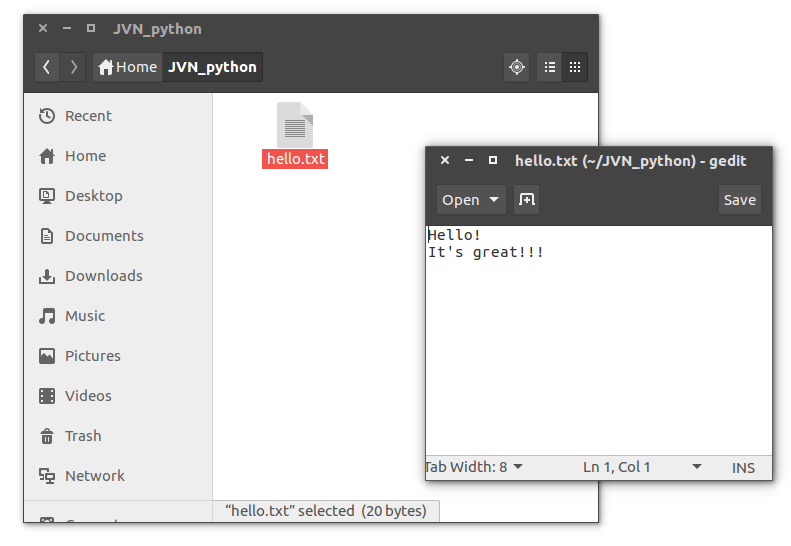
\includegraphics{figs/session_4/write_file_demo.png}
\caption{}
\end{figure}

    The \textbf{read()} method reads a string from an open file. It is
important to note that Python strings can have binary data. apart from
text data.

Syntax

\begin{verbatim}
fileObject.read([count]);
\end{verbatim}

Here, passed parameter is the number of bytes to be read from the opened
file. This method starts reading from the beginning of the file and if
count is missing, then it tries to read as much as possible, maybe until
the end of file.

Example

Let's take a file hello.txt, which we created above.

    \begin{Verbatim}[commandchars=\\\{\}]
{\color{incolor}In [{\color{incolor}35}]:} \PY{n}{f} \PY{o}{=} \PY{n+nb}{open}\PY{p}{(}\PY{l+s+s2}{\PYZdq{}}\PY{l+s+s2}{hello.txt}\PY{l+s+s2}{\PYZdq{}}\PY{p}{,} \PY{l+s+s2}{\PYZdq{}}\PY{l+s+s2}{r+}\PY{l+s+s2}{\PYZdq{}}\PY{p}{)}
         \PY{k}{print} \PY{n}{f}\PY{o}{.}\PY{n}{read}\PY{p}{(}\PY{p}{)}
         \PY{n}{f}\PY{o}{.}\PY{n}{close}\PY{p}{(}\PY{p}{)}
\end{Verbatim}

    \begin{Verbatim}[commandchars=\\\{\}]
Hello!
It's great!!!

    \end{Verbatim}

    \subsection{Renaming and Deleting
Files}\label{renaming-and-deleting-files}

Python \textbf{os} module provides methods that help you perform
file-processing operations, such as renaming and deleting files.

To use this module you need to import it first and then you can call any
related functions.

    \subsubsection{The rename() Method}\label{the-rename-method}

The \textbf{rename()} method takes two arguments, the current filename
and the new filename:

\begin{Shaded}
\begin{Highlighting}[]
\NormalTok{os.rename(current_file_name, new_file_name)}
\end{Highlighting}
\end{Shaded}

    \begin{Verbatim}[commandchars=\\\{\}]
{\color{incolor}In [{\color{incolor}36}]:} \PY{k+kn}{import} \PY{n+nn}{os}
         
         \PY{n}{os}\PY{o}{.}\PY{n}{rename}\PY{p}{(}\PY{l+s+s2}{\PYZdq{}}\PY{l+s+s2}{hello.txt}\PY{l+s+s2}{\PYZdq{}}\PY{p}{,} \PY{l+s+s2}{\PYZdq{}}\PY{l+s+s2}{hi.txt}\PY{l+s+s2}{\PYZdq{}}\PY{p}{)}
\end{Verbatim}

    \subsubsection{The remove() Method}\label{the-remove-method}

You can use the \textbf{remove()} method to delete files by supplying
the name of the file to be deleted as the argument.

Syntax

\begin{Shaded}
\begin{Highlighting}[]
\NormalTok{os.remove(file_name)}
\end{Highlighting}
\end{Shaded}

    \begin{Verbatim}[commandchars=\\\{\}]
{\color{incolor}In [{\color{incolor}37}]:} \PY{k+kn}{import} \PY{n+nn}{os}
         
         \PY{n}{os}\PY{o}{.}\PY{n}{remove}\PY{p}{(}\PY{l+s+s2}{\PYZdq{}}\PY{l+s+s2}{hi.txt}\PY{l+s+s2}{\PYZdq{}}\PY{p}{)}
\end{Verbatim}

    \begin{Verbatim}[commandchars=\\\{\}]
{\color{incolor}In [{\color{incolor}38}]:} \PY{c+c1}{\PYZsh{} Remove not exsists file}
         
         \PY{n}{os}\PY{o}{.}\PY{n}{remove}\PY{p}{(}\PY{l+s+s2}{\PYZdq{}}\PY{l+s+s2}{some\PYZus{}file.txt}\PY{l+s+s2}{\PYZdq{}}\PY{p}{)}
\end{Verbatim}

    \begin{Verbatim}[commandchars=\\\{\}]

        ---------------------------------------------------------------------------

        OSError                                   Traceback (most recent call last)

        <ipython-input-38-6b72632a7e6b> in <module>()
          1 \# Remove not exsists file
          2 
    ----> 3 os.remove("some\_file.txt")
    

        OSError: [Errno 2] No such file or directory: 'some\_file.txt'

    \end{Verbatim}

    \subsection{Directories in Python}\label{directories-in-python}

The \textbf{os} module has several methods that help you create, remove,
and change directories.

\subsubsection{The mkdir() Method}\label{the-mkdir-method}

You can use the mkdir() method of the os module to create directories in
the current directory

\begin{Shaded}
\begin{Highlighting}[]
\NormalTok{os.mkdir(}\StringTok{"newdir"}\NormalTok{)}
\end{Highlighting}
\end{Shaded}

    \begin{Verbatim}[commandchars=\\\{\}]
{\color{incolor}In [{\color{incolor}39}]:} \PY{n}{os}\PY{o}{.}\PY{n}{mkdir}\PY{p}{(}\PY{l+s+s2}{\PYZdq{}}\PY{l+s+s2}{duyet}\PY{l+s+s2}{\PYZdq{}}\PY{p}{)}
\end{Verbatim}

    \begin{figure}
\centering
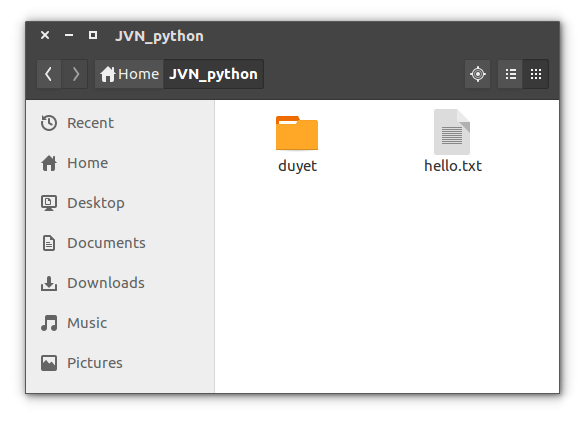
\includegraphics{figs/session_4/mkdir.png}
\caption{}
\end{figure}

    \subsubsection{The chdir() Method}\label{the-chdir-method}

You can use the \textbf{chdir()} method to change the current directory.

\begin{Shaded}
\begin{Highlighting}[]
\NormalTok{os.chdir(}\StringTok{"newdir"}\NormalTok{)}
\end{Highlighting}
\end{Shaded}

    \subsubsection{The getcwd() Method}\label{the-getcwd-method}

The \textbf{getcwd()} method displays the current working directory.

    \begin{Verbatim}[commandchars=\\\{\}]
{\color{incolor}In [{\color{incolor}41}]:} \PY{k}{print} \PY{n}{os}\PY{o}{.}\PY{n}{getcwd}\PY{p}{(}\PY{p}{)}
\end{Verbatim}

    \begin{Verbatim}[commandchars=\\\{\}]
/home/duyetdev/project/Python-R-Basic

    \end{Verbatim}

    \subsubsection{The rmdir() Method}\label{the-rmdir-method}

The rmdir() method deletes the directory, which is passed as an argument
in the method.

\begin{Shaded}
\begin{Highlighting}[]
\NormalTok{os.rmdir(}\StringTok{'dirname'}\NormalTok{)}
\end{Highlighting}
\end{Shaded}

    \begin{Verbatim}[commandchars=\\\{\}]
{\color{incolor}In [{\color{incolor}50}]:} \PY{n}{os}\PY{o}{.}\PY{n}{rmdir}\PY{p}{(}\PY{l+s+s2}{\PYZdq{}}\PY{l+s+s2}{./duyet}\PY{l+s+s2}{\PYZdq{}}\PY{p}{)}
\end{Verbatim}

    \begin{Verbatim}[commandchars=\\\{\}]
{\color{incolor}In [{\color{incolor} }]:} 
\end{Verbatim}

    \begin{Verbatim}[commandchars=\\\{\}]
{\color{incolor}In [{\color{incolor} }]:} 
\end{Verbatim}

    \textbf{Ex:} Creates the following folder structure

    \section{Pandas}\label{pandas}

Pandas is a package of fast, efficient data analysis tools for Python

Just as NumPy provides the basic array data type plus core array
operations, pandas

\begin{itemize}
\tightlist
\item
  defines fundamental structures for working with data and
\item
  endows them with methods that facilitate operations such as

  \begin{itemize}
  \tightlist
  \item
    reading in data
  \item
    adjusting indices
  \item
    working with dates and time series
  \item
    sorting, grouping, re-ordering and general data munging {[}1{]}
  \item
    dealing with missing values, etc., etc.
  \end{itemize}
\end{itemize}

More sophisticated statistical functionality is left to other packages,
such as statsmodels and scikit-learn, which are built on top of pandas

    \begin{Verbatim}[commandchars=\\\{\}]
{\color{incolor}In [{\color{incolor}52}]:} \PY{k+kn}{import} \PY{n+nn}{numpy} \PY{k+kn}{as} \PY{n+nn}{np}
         \PY{k+kn}{import} \PY{n+nn}{pandas} \PY{k+kn}{as} \PY{n+nn}{pd}
\end{Verbatim}

    \subsection{Series}\label{series}

Two important data types defined by pandas are \textbf{Series} and
\textbf{DataFrame}

You can think of a Series as a ``column'' of data, such as a collection
of observations on a single variable

A DataFrame is an object for storing related columns of data

Let's start with Series

    \begin{Verbatim}[commandchars=\\\{\}]
{\color{incolor}In [{\color{incolor}53}]:} \PY{n}{s} \PY{o}{=} \PY{n}{pd}\PY{o}{.}\PY{n}{Series}\PY{p}{(}\PY{n}{np}\PY{o}{.}\PY{n}{random}\PY{o}{.}\PY{n}{randn}\PY{p}{(}\PY{l+m+mi}{4}\PY{p}{)}\PY{p}{,} \PY{n}{name}\PY{o}{=}\PY{l+s+s1}{\PYZsq{}}\PY{l+s+s1}{daily returns}\PY{l+s+s1}{\PYZsq{}}\PY{p}{)}
         \PY{n}{s}
\end{Verbatim}

            \begin{Verbatim}[commandchars=\\\{\}]
{\color{outcolor}Out[{\color{outcolor}53}]:} 0    0.109632
         1    0.125849
         2    1.593836
         3   -1.826518
         Name: daily returns, dtype: float64
\end{Verbatim}
        
    Here you can imagine the indices \texttt{0,\ 1,\ 2,\ 3} as
\textbf{indexing} four listed companies, and the values being daily
returns on their shares.

Pandas \textbf{Series} are built on top of NumPy arrays, and support
many similar operations

    \begin{Verbatim}[commandchars=\\\{\}]
{\color{incolor}In [{\color{incolor}54}]:} \PY{n}{s} \PY{o}{*} \PY{l+m+mi}{100}
\end{Verbatim}

            \begin{Verbatim}[commandchars=\\\{\}]
{\color{outcolor}Out[{\color{outcolor}54}]:} 0     10.963232
         1     12.584910
         2    159.383605
         3   -182.651820
         Name: daily returns, dtype: float64
\end{Verbatim}
        
    \begin{Verbatim}[commandchars=\\\{\}]
{\color{incolor}In [{\color{incolor}55}]:} \PY{n}{s}\PY{o}{.}\PY{n}{abs}\PY{p}{(}\PY{p}{)}
\end{Verbatim}

            \begin{Verbatim}[commandchars=\\\{\}]
{\color{outcolor}Out[{\color{outcolor}55}]:} 0    0.109632
         1    0.125849
         2    1.593836
         3    1.826518
         Name: daily returns, dtype: float64
\end{Verbatim}
        
    \begin{Verbatim}[commandchars=\\\{\}]
{\color{incolor}In [{\color{incolor}57}]:} \PY{n}{s}\PY{p}{[}\PY{n}{s} \PY{o}{\PYZgt{}}\PY{o}{=} \PY{l+m+mi}{1}\PY{p}{]}
\end{Verbatim}

            \begin{Verbatim}[commandchars=\\\{\}]
{\color{outcolor}Out[{\color{outcolor}57}]:} 2    1.593836
         Name: daily returns, dtype: float64
\end{Verbatim}
        
    \begin{Verbatim}[commandchars=\\\{\}]
{\color{incolor}In [{\color{incolor}58}]:} \PY{n}{s}\PY{o}{.}\PY{n}{describe}\PY{p}{(}\PY{p}{)}
\end{Verbatim}

            \begin{Verbatim}[commandchars=\\\{\}]
{\color{outcolor}Out[{\color{outcolor}58}]:} count    4.000000
         mean     0.000700
         std      1.402894
         min     -1.826518
         25\%     -0.374405
         50\%      0.117741
         75\%      0.492846
         max      1.593836
         Name: daily returns, dtype: float64
\end{Verbatim}
        
    But their indices are more flexible

    \begin{Verbatim}[commandchars=\\\{\}]
{\color{incolor}In [{\color{incolor}59}]:} \PY{n}{s}\PY{o}{.}\PY{n}{index} \PY{o}{=} \PY{p}{[}\PY{l+s+s1}{\PYZsq{}}\PY{l+s+s1}{AMZN}\PY{l+s+s1}{\PYZsq{}}\PY{p}{,} \PY{l+s+s1}{\PYZsq{}}\PY{l+s+s1}{AAPL}\PY{l+s+s1}{\PYZsq{}}\PY{p}{,} \PY{l+s+s1}{\PYZsq{}}\PY{l+s+s1}{MSFT}\PY{l+s+s1}{\PYZsq{}}\PY{p}{,} \PY{l+s+s1}{\PYZsq{}}\PY{l+s+s1}{GOOG}\PY{l+s+s1}{\PYZsq{}}\PY{p}{]}
         \PY{n}{s}
\end{Verbatim}

            \begin{Verbatim}[commandchars=\\\{\}]
{\color{outcolor}Out[{\color{outcolor}59}]:} AMZN    0.109632
         AAPL    0.125849
         MSFT    1.593836
         GOOG   -1.826518
         Name: daily returns, dtype: float64
\end{Verbatim}
        
    \begin{Verbatim}[commandchars=\\\{\}]
{\color{incolor}In [{\color{incolor}60}]:} \PY{n}{s}\PY{p}{[}\PY{l+s+s1}{\PYZsq{}}\PY{l+s+s1}{GOOG}\PY{l+s+s1}{\PYZsq{}}\PY{p}{]}
\end{Verbatim}

            \begin{Verbatim}[commandchars=\\\{\}]
{\color{outcolor}Out[{\color{outcolor}60}]:} -1.8265181959162498
\end{Verbatim}
        
    \subsection{DataFrames}\label{dataframes}

While a Series is a single column of data, a DataFrame is several
columns, one for each variable.

Here's the contents of \emph{test\_pwt.csv}

\begin{verbatim}
"country","country isocode","year","POP","XRAT","tcgdp","cc","cg"
"Argentina","ARG","2000","37335.653","0.9995","295072.21869","75.716805379","5.5788042896"
"Australia","AUS","2000","19053.186","1.72483","541804.6521","67.759025993","6.7200975332"
"India","IND","2000","1006300.297","44.9416","1728144.3748","64.575551328","14.072205773"
"Israel","ISR","2000","6114.57","4.07733","129253.89423","64.436450847","10.266688415"
"Malawi","MWI","2000","11801.505","59.543808333","5026.2217836","74.707624181","11.658954494"
"South Africa","ZAF","2000","45064.098","6.93983","227242.36949","72.718710427","5.7265463933"
"United States","USA","2000","282171.957","1","9898700","72.347054303","6.0324539789"
"Uruguay","URY","2000","3219.793","12.099591667","25255.961693","78.978740282","5.108067988"
\end{verbatim}

    \begin{Verbatim}[commandchars=\\\{\}]
{\color{incolor}In [{\color{incolor}61}]:} \PY{n}{df} \PY{o}{=} \PY{n}{pd}\PY{o}{.}\PY{n}{read\PYZus{}csv}\PY{p}{(}\PY{l+s+s1}{\PYZsq{}}\PY{l+s+s1}{https://github.com/QuantEcon/QuantEcon.lectures.code/raw/master/pandas/data/test\PYZus{}pwt.csv}\PY{l+s+s1}{\PYZsq{}}\PY{p}{)}
\end{Verbatim}

    \begin{Verbatim}[commandchars=\\\{\}]
{\color{incolor}In [{\color{incolor}62}]:} \PY{n}{df}\PY{o}{.}\PY{n}{head}\PY{p}{(}\PY{p}{)}
\end{Verbatim}

            \begin{Verbatim}[commandchars=\\\{\}]
{\color{outcolor}Out[{\color{outcolor}62}]:}      country country isocode  year          POP       XRAT         tcgdp  \textbackslash{}
         0  Argentina             ARG  2000    37335.653   0.999500  2.950722e+05   
         1  Australia             AUS  2000    19053.186   1.724830  5.418047e+05   
         2      India             IND  2000  1006300.297  44.941600  1.728144e+06   
         3     Israel             ISR  2000     6114.570   4.077330  1.292539e+05   
         4     Malawi             MWI  2000    11801.505  59.543808  5.026222e+03   
         
                   cc         cg  
         0  75.716805   5.578804  
         1  67.759026   6.720098  
         2  64.575551  14.072206  
         3  64.436451  10.266688  
         4  74.707624  11.658954  
\end{Verbatim}
        
    \begin{Verbatim}[commandchars=\\\{\}]
{\color{incolor}In [{\color{incolor}63}]:} \PY{n}{df}\PY{p}{[}\PY{l+m+mi}{2}\PY{p}{:}\PY{l+m+mi}{4}\PY{p}{]}
\end{Verbatim}

            \begin{Verbatim}[commandchars=\\\{\}]
{\color{outcolor}Out[{\color{outcolor}63}]:}   country country isocode  year          POP      XRAT         tcgdp  \textbackslash{}
         2   India             IND  2000  1006300.297  44.94160  1.728144e+06   
         3  Israel             ISR  2000     6114.570   4.07733  1.292539e+05   
         
                   cc         cg  
         2  64.575551  14.072206  
         3  64.436451  10.266688  
\end{Verbatim}
        
    To select columns, we can pass a list containing the names of the
desired columns represented as strings

    \begin{Verbatim}[commandchars=\\\{\}]
{\color{incolor}In [{\color{incolor}64}]:} \PY{n}{df}\PY{p}{[}\PY{p}{[}\PY{l+s+s1}{\PYZsq{}}\PY{l+s+s1}{country}\PY{l+s+s1}{\PYZsq{}}\PY{p}{,} \PY{l+s+s1}{\PYZsq{}}\PY{l+s+s1}{tcgdp}\PY{l+s+s1}{\PYZsq{}}\PY{p}{]}\PY{p}{]}
\end{Verbatim}

            \begin{Verbatim}[commandchars=\\\{\}]
{\color{outcolor}Out[{\color{outcolor}64}]:}          country         tcgdp
         0      Argentina  2.950722e+05
         1      Australia  5.418047e+05
         2          India  1.728144e+06
         3         Israel  1.292539e+05
         4         Malawi  5.026222e+03
         5   South Africa  2.272424e+05
         6  United States  9.898700e+06
         7        Uruguay  2.525596e+04
\end{Verbatim}
        
    To select both rows and columns using integers, the iloc attribute
should be used with the format \texttt{.iloc{[}rows,columns{]}}

    \begin{Verbatim}[commandchars=\\\{\}]
{\color{incolor}In [{\color{incolor}65}]:} \PY{n}{df}\PY{o}{.}\PY{n}{iloc}\PY{p}{[}\PY{l+m+mi}{2}\PY{p}{:}\PY{l+m+mi}{5}\PY{p}{,}\PY{l+m+mi}{0}\PY{p}{:}\PY{l+m+mi}{4}\PY{p}{]}
\end{Verbatim}

            \begin{Verbatim}[commandchars=\\\{\}]
{\color{outcolor}Out[{\color{outcolor}65}]:}   country country isocode  year          POP
         2   India             IND  2000  1006300.297
         3  Israel             ISR  2000     6114.570
         4  Malawi             MWI  2000    11801.505
\end{Verbatim}
        
    To select rows and columns using a mixture of integers and labels, the
loc attribute can be used in a similar way

    \begin{Verbatim}[commandchars=\\\{\}]
{\color{incolor}In [{\color{incolor}70}]:} \PY{n}{df}\PY{o}{.}\PY{n}{loc}\PY{p}{[}\PY{n}{df}\PY{o}{.}\PY{n}{index}\PY{p}{[}\PY{l+m+mi}{2}\PY{p}{:}\PY{l+m+mi}{5}\PY{p}{]}\PY{p}{,} \PY{p}{[}\PY{l+s+s1}{\PYZsq{}}\PY{l+s+s1}{year}\PY{l+s+s1}{\PYZsq{}}\PY{p}{,} \PY{l+s+s1}{\PYZsq{}}\PY{l+s+s1}{country}\PY{l+s+s1}{\PYZsq{}}\PY{p}{]}\PY{p}{]}
\end{Verbatim}

            \begin{Verbatim}[commandchars=\\\{\}]
{\color{outcolor}Out[{\color{outcolor}70}]:}    year country
         2  2000   India
         3  2000  Israel
         4  2000  Malawi
\end{Verbatim}
        
    Let's imagine that we're only interested in population and total
\texttt{GDP} (tcgdp).

One way to strip the data frame df down to only these variables is to
overwrite the dataframe using the selection method described above

    \begin{Verbatim}[commandchars=\\\{\}]
{\color{incolor}In [{\color{incolor}71}]:} \PY{n}{df} \PY{o}{=} \PY{n}{df}\PY{p}{[}\PY{p}{[}\PY{l+s+s1}{\PYZsq{}}\PY{l+s+s1}{country}\PY{l+s+s1}{\PYZsq{}}\PY{p}{,}\PY{l+s+s1}{\PYZsq{}}\PY{l+s+s1}{POP}\PY{l+s+s1}{\PYZsq{}}\PY{p}{,}\PY{l+s+s1}{\PYZsq{}}\PY{l+s+s1}{tcgdp}\PY{l+s+s1}{\PYZsq{}}\PY{p}{]}\PY{p}{]}
         \PY{n}{df}
\end{Verbatim}

            \begin{Verbatim}[commandchars=\\\{\}]
{\color{outcolor}Out[{\color{outcolor}71}]:}          country          POP         tcgdp
         0      Argentina    37335.653  2.950722e+05
         1      Australia    19053.186  5.418047e+05
         2          India  1006300.297  1.728144e+06
         3         Israel     6114.570  1.292539e+05
         4         Malawi    11801.505  5.026222e+03
         5   South Africa    45064.098  2.272424e+05
         6  United States   282171.957  9.898700e+06
         7        Uruguay     3219.793  2.525596e+04
\end{Verbatim}
        
    Here the index 0, 1,..., 7 is redundant, because we can use the country
names as an index

To do this, we set the index to be the country variable in the dataframe

    \begin{Verbatim}[commandchars=\\\{\}]
{\color{incolor}In [{\color{incolor}72}]:} \PY{n}{df} \PY{o}{=} \PY{n}{df}\PY{o}{.}\PY{n}{set\PYZus{}index}\PY{p}{(}\PY{l+s+s1}{\PYZsq{}}\PY{l+s+s1}{country}\PY{l+s+s1}{\PYZsq{}}\PY{p}{)}
         \PY{n}{df}
\end{Verbatim}

            \begin{Verbatim}[commandchars=\\\{\}]
{\color{outcolor}Out[{\color{outcolor}72}]:}                        POP         tcgdp
         country                                 
         Argentina        37335.653  2.950722e+05
         Australia        19053.186  5.418047e+05
         India          1006300.297  1.728144e+06
         Israel            6114.570  1.292539e+05
         Malawi           11801.505  5.026222e+03
         South Africa     45064.098  2.272424e+05
         United States   282171.957  9.898700e+06
         Uruguay           3219.793  2.525596e+04
\end{Verbatim}
        
    \begin{Verbatim}[commandchars=\\\{\}]
{\color{incolor}In [{\color{incolor}73}]:} \PY{n}{df}\PY{o}{.}\PY{n}{columns} \PY{o}{=} \PY{l+s+s1}{\PYZsq{}}\PY{l+s+s1}{population}\PY{l+s+s1}{\PYZsq{}}\PY{p}{,} \PY{l+s+s1}{\PYZsq{}}\PY{l+s+s1}{total GDP}\PY{l+s+s1}{\PYZsq{}}
         \PY{n}{df}
\end{Verbatim}

            \begin{Verbatim}[commandchars=\\\{\}]
{\color{outcolor}Out[{\color{outcolor}73}]:}                 population     total GDP
         country                                 
         Argentina        37335.653  2.950722e+05
         Australia        19053.186  5.418047e+05
         India          1006300.297  1.728144e+06
         Israel            6114.570  1.292539e+05
         Malawi           11801.505  5.026222e+03
         South Africa     45064.098  2.272424e+05
         United States   282171.957  9.898700e+06
         Uruguay           3219.793  2.525596e+04
\end{Verbatim}
        
    Population is in thousands, let's revert to single units

    \begin{Verbatim}[commandchars=\\\{\}]
{\color{incolor}In [{\color{incolor}74}]:} \PY{n}{df}\PY{p}{[}\PY{l+s+s1}{\PYZsq{}}\PY{l+s+s1}{population}\PY{l+s+s1}{\PYZsq{}}\PY{p}{]} \PY{o}{=} \PY{n}{df}\PY{p}{[}\PY{l+s+s1}{\PYZsq{}}\PY{l+s+s1}{population}\PY{l+s+s1}{\PYZsq{}}\PY{p}{]} \PY{o}{*} \PY{l+m+mf}{1e3}
         \PY{n}{df}
\end{Verbatim}

            \begin{Verbatim}[commandchars=\\\{\}]
{\color{outcolor}Out[{\color{outcolor}74}]:}                  population     total GDP
         country                                  
         Argentina      3.733565e+07  2.950722e+05
         Australia      1.905319e+07  5.418047e+05
         India          1.006300e+09  1.728144e+06
         Israel         6.114570e+06  1.292539e+05
         Malawi         1.180150e+07  5.026222e+03
         South Africa   4.506410e+07  2.272424e+05
         United States  2.821720e+08  9.898700e+06
         Uruguay        3.219793e+06  2.525596e+04
\end{Verbatim}
        
    Next we're going to add a column showing real GDP per capita,
multiplying by 1,000,000 as we go because total GDP is in millions

    \begin{Verbatim}[commandchars=\\\{\}]
{\color{incolor}In [{\color{incolor}75}]:} \PY{n}{df}\PY{p}{[}\PY{l+s+s1}{\PYZsq{}}\PY{l+s+s1}{GDP percap}\PY{l+s+s1}{\PYZsq{}}\PY{p}{]} \PY{o}{=} \PY{n}{df}\PY{p}{[}\PY{l+s+s1}{\PYZsq{}}\PY{l+s+s1}{total GDP}\PY{l+s+s1}{\PYZsq{}}\PY{p}{]} \PY{o}{*} \PY{l+m+mf}{1e6} \PY{o}{/} \PY{n}{df}\PY{p}{[}\PY{l+s+s1}{\PYZsq{}}\PY{l+s+s1}{population}\PY{l+s+s1}{\PYZsq{}}\PY{p}{]}
         \PY{n}{df}
\end{Verbatim}

            \begin{Verbatim}[commandchars=\\\{\}]
{\color{outcolor}Out[{\color{outcolor}75}]:}                  population     total GDP    GDP percap
         country                                                
         Argentina      3.733565e+07  2.950722e+05   7903.229085
         Australia      1.905319e+07  5.418047e+05  28436.433261
         India          1.006300e+09  1.728144e+06   1717.324719
         Israel         6.114570e+06  1.292539e+05  21138.672749
         Malawi         1.180150e+07  5.026222e+03    425.896679
         South Africa   4.506410e+07  2.272424e+05   5042.647686
         United States  2.821720e+08  9.898700e+06  35080.381854
         Uruguay        3.219793e+06  2.525596e+04   7843.970620
\end{Verbatim}
        
    One of the nice things about pandas DataFrame and Series objects is that
they have methods for plotting and visualization that work through
Matplotlib

    \begin{Verbatim}[commandchars=\\\{\}]
{\color{incolor}In [{\color{incolor}77}]:} \PY{n}{df}\PY{p}{[}\PY{l+s+s1}{\PYZsq{}}\PY{l+s+s1}{GDP percap}\PY{l+s+s1}{\PYZsq{}}\PY{p}{]}\PY{o}{.}\PY{n}{plot}\PY{p}{(}\PY{n}{kind}\PY{o}{=}\PY{l+s+s1}{\PYZsq{}}\PY{l+s+s1}{bar}\PY{l+s+s1}{\PYZsq{}}\PY{p}{)}
\end{Verbatim}

            \begin{Verbatim}[commandchars=\\\{\}]
{\color{outcolor}Out[{\color{outcolor}77}]:} <matplotlib.axes.\_subplots.AxesSubplot at 0x7f230ff42650>
\end{Verbatim}
        
    \begin{Verbatim}[commandchars=\\\{\}]
{\color{incolor}In [{\color{incolor}78}]:} \PY{k+kn}{import} \PY{n+nn}{matplotlib.pyplot} \PY{k+kn}{as} \PY{n+nn}{plt}
         
         \PY{n}{plt}\PY{o}{.}\PY{n}{show}\PY{p}{(}\PY{p}{)}
\end{Verbatim}

    \begin{center}
    \adjustimage{max size={0.9\linewidth}{0.9\paperheight}}{output_61_0.png}
    \end{center}
    { \hspace*{\fill} \\}
    
    \section{References}\label{references}

\begin{itemize}
\tightlist
\item
  10 Minutes to pandas -
  (https://pandas.pydata.org/pandas-docs/stable/10min.html){[}https://pandas.pydata.org/pandas-docs/stable/10min.html{]}
\item
  Pandas Tutorial: DataFrames in Python
  \url{https://www.datacamp.com/community/tutorials/pandas-tutorial-dataframe-python}
\item
  \url{https://www.tutorialspoint.com/python/python_files_io.htm}
\end{itemize}

    \section{Excercises}\label{excercises}

\textbf{Python Program to Merge Mails}

When we want to send the same invitations to many people, the body of
the mail does not change. Only the name (and maybe address) needs to be
changed.

Mail merge is a process of doing this. Instead of writing each mail
separately, we have a template for body of the mail and a list of names
that we merge together to form all the mails.

For this program, we have written all the names and emails in separate
lines in the file "names.csv". The body is in the "body.txt" file.

\begin{figure}
\centering
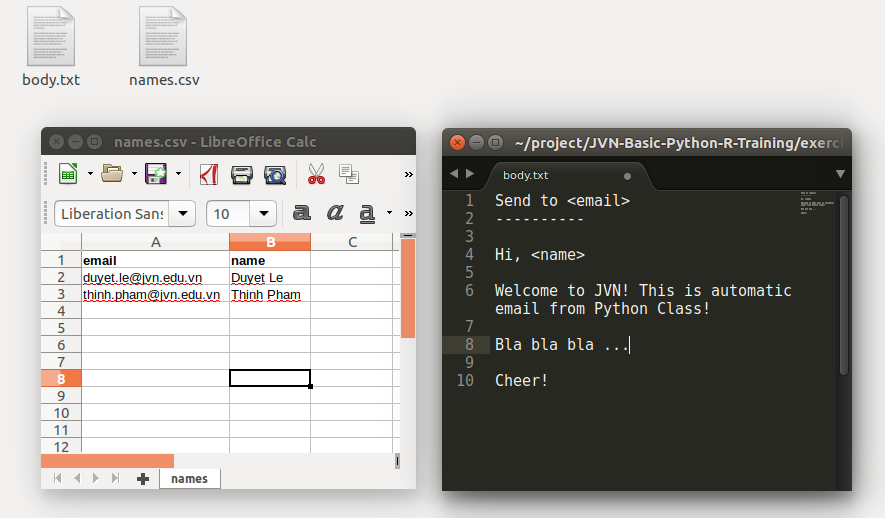
\includegraphics{figs/session_4/merge_mails.png}
\caption{figs/session\_4/merge\_mails.png}
\end{figure}

We open both the files in reading mode and iterate over each name. A new
file with the name "{[}name{]}.txt" is created, where name is the name
of that person. Replace the and in body email.

    \begin{Verbatim}[commandchars=\\\{\}]
{\color{incolor}In [{\color{incolor} }]:} 
\end{Verbatim}


    % Add a bibliography block to the postdoc
    
    
    
    \end{document}
